\section{Ajout de fonctionnalités}

\subsection{L'implémentation du retour sonore}
\paragraph{}
Dans le programme de Jérémy Lixandre, la classe \verb!Parser! a pour
utilité de récupérer les informations du fichier de configuration
\verb!config.cfg!, notamment toutes les fonctions de
\textit{processing}. Ce fichier a donc été modifié afin de prendre en
compte notre nouvelle fonction de \textit{processing}, la fonction de
mixage, qui vient s'ajouter aux trois existantes. Tout comme ces
fonctions, elle est générique et doit pouvoir être sélectionnée par
l'utilisateur depuis un menu de configuration.

\paragraph{}
Un fichier dédié à la fonction de mixage a un nom commençant par
\verb!Mix!. Il est répertorié dans le dossier \verb!Mix! du dossier
\verb!Process!. La fonction de mixage doit prendre une matrice en
paramètre ; il s'agit de la matrice retournée par la fonction de
calcul du coefficient de corrélation. Elle retourne un vecteur de
coefficients : à un instant donné, chaque piste dispose désormais d'un
seul coefficient qui doit déterminer la façon dont elle va être
diminuée en volume sonore dans le retour audio.

\paragraph{}
Nous avons implémenté plusieurs fonctions de mixage. La fonction
\verb!vector<float>!
\\ \verb!MixMaxCorrelated(const Matrix<float>& correlMatrix)!, par
exemple, renvoie un coefficient égal à la moyenne des coefficients de
corrélation de la piste avec toutes les autres pistes. Tandis que la
fonction de traduction du coefficient de corrélation en triplet RGB
est dédiée uniquement au retour visuel, celle de mixage est dédiée
uniquement au retour sonore.

\begin{lstlisting}
vector<float> MixMaxCorrelated(const Matrix<float>& correlMatrix) {

  int row = correlMatrix.getSize();
  int col = correlMatrix.getRow(0).size();

  // initialize the result vector with zeros
  vector<float> meanCorrelations(row, 0.0f);

  // fill the vector with the mean correlation of each instrument with others
  for (int i = 0; i < row; i++) {
    for (int j = 0; j < col; j++) {
      if (i != j)
        meanCorrelations[i] += correlMatrix.getCase(i, j);
    }
    meanCorrelations[i] /= (float)row-1;
  }

  return meanCorrelations;
}
}
\end{lstlisting}

\begin{center}
 \textit{Ci-dessus, l'exemple de la fonction de mixage précédemment cité}
\end{center}

\paragraph{}
Dans la fonction
\verb!void parseProcessFunc(ChSettings& gChSettings, const!
\\ \verb!Parser& config, ProcessMultiCorrel *p, void *handle)!
appelée dans le fichier \\ \verb!main.cpp!, nous avons dû ajouter
l'analyse de la fonction de mixage sur le modèle des analyses des
trois autres fonctions de \textit{processing}.

\paragraph{}
L'architecture de Bela a été conçue pour permettre la synthèse d'un
retour sonore dans le corps de la fonction
\verb!void render(BelaContext *context, void *userData)! du fichier
éponyme. Grâce au code implémenté par notre prédécesseur au sein de
cette fonction, Bela peut synthétiser un retour sonore modifié par
notre fonction de mixage.

\begin{lstlisting} for(unsigned int i=0; i<context->audioOutChannels; i++){ if
(gSampleFactor == STANDARD_SAMPLE_RATE) { audioWrite(context, 2 * n, i, out);
audioWrite(context, 2 * n + 1, i, out); } else { audioWrite(context, n, i, out); } }
\end{lstlisting} \begin{center} Ci-dessus, l'implémentation du retour sonore
dans le corps de la fonction principale de \verb!render.cpp! \end{center}

\paragraph{}
Dans le fichier \verb!render.cpp!, la fonction
\verb!void processBuffer()! est utilisée comme tâche auxiliaire de la
boucle de traitement principale. Nous avons déclaré un vecteur
\verb!gMeanCorrel! dans \verb!render.cpp! ; initialisé avec une valeur
de 1 pour tous les indices, il prend la valeur que retourne la
fonction de mixage à l'intérieur du code de la fonction
\verb!void ProcessMultiCorrel::process(const Matrix<float>& buffer,! \\ \verb!vector<float>& meanCorrelations, Connection conn)!
que nous avons modifiée et qui est appelée dans \verb!processBuffer!
de \verb!render.cpp!.

\subsection{L'interface de configuration utilisateur}
\paragraph{}
Afin d'implémenter l'interface de configuration utilisateur précédemment abordée
nous avons ajouté à l'architecture du programme un dossier
\verb!GUI! (\textit{Graphic User Interface}) à la racine du programme.
Le sous-répertoire contenant les fichiers relatifs à l'implémentation de
l'interface de configuration se nomme \verb!settingWindow!.

\begin{figure}[h]
 \centering
 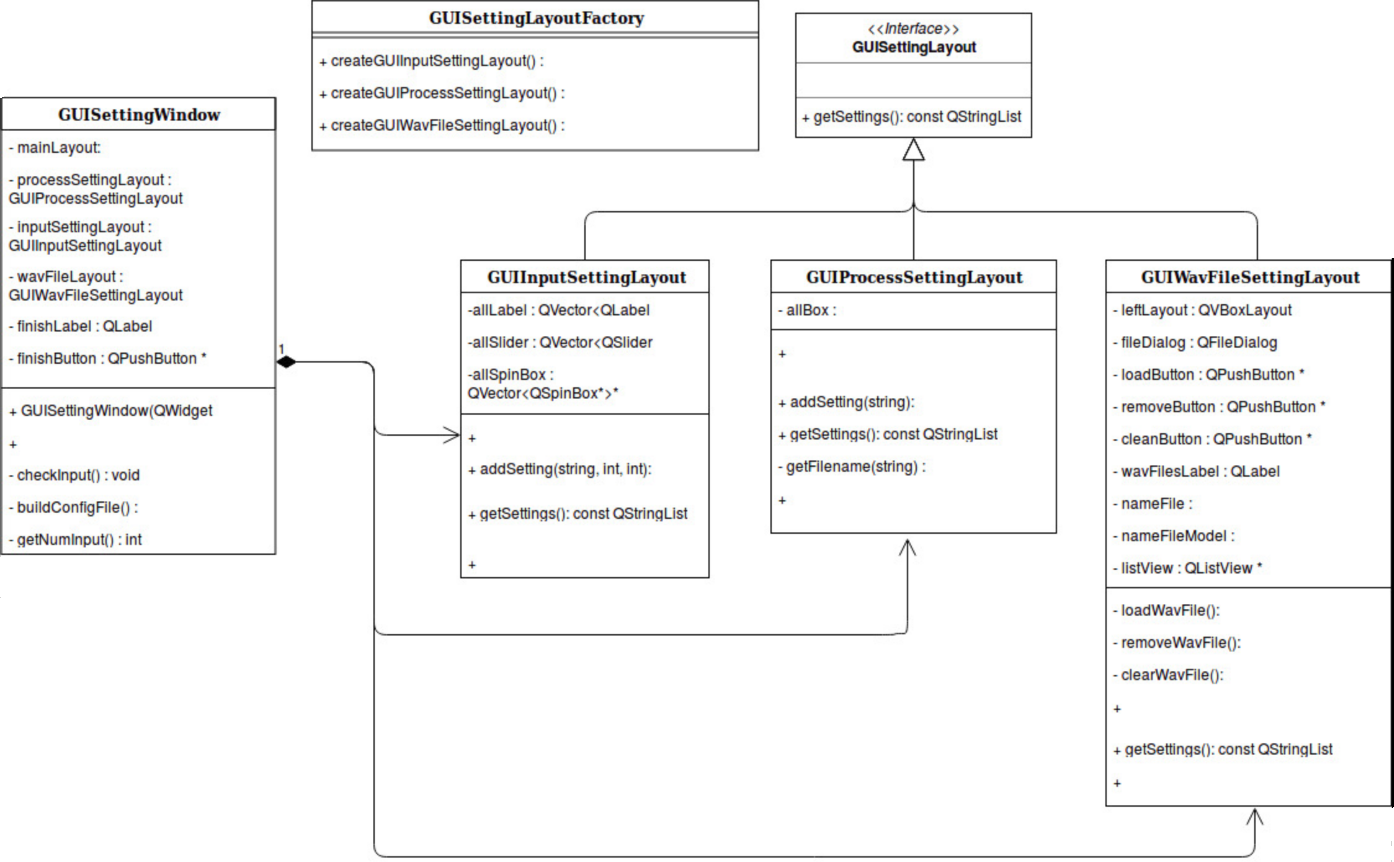
\includegraphics[scale=0.3]{umlSettingWindow.png}
 \verb!\caption{Schéma global du dispositif de VisualImpro}!
 \label{schéma global}
\end{figure}

\paragraph{}
La fenêtre de configuration

\begin{figure}[h]
 \centering
 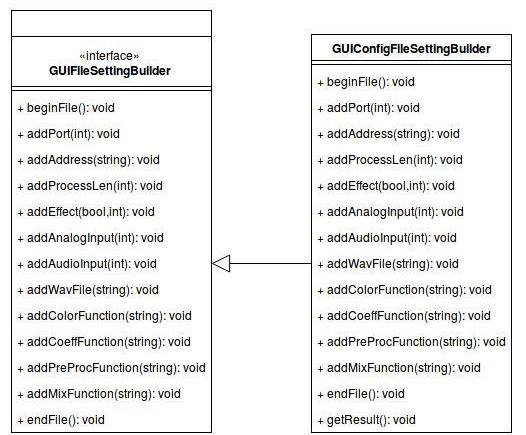
\includegraphics[scale=0.5]{umlBuilder.png}
 \verb!\caption{Schéma global du dispositif de VisualImpro}!
 \label{schéma global}
\end{figure}

\paragraph{}
La fenêtre de configuration

\subsection{Autres ajouts mineurs sur le programme}
